\documentclass[sigconf]{acmart}

%% Rights management
\setcopyright{none}
\acmConference[AI4HPCC '26]{Workshop on AI for High Performance Compiler Construction}{July 6--9, 2026}{Belfast, Northern Ireland, UK}

\usepackage{booktabs}
\usepackage{subcaption}
\usepackage{xspace}
\usepackage{listings}
\usepackage{xcolor}
\usepackage{tikz}
\usetikzlibrary{arrows.meta,positioning,shapes.geometric,fit}

\lstset{
  basicstyle=\ttfamily\scriptsize,
  keywordstyle=\color{blue}\bfseries,
  commentstyle=\color{gray},
  stringstyle=\color{red},
  breaklines=true,
  frame=single,
  columns=fullflexible,
  keepspaces=true,
  numbers=left,
  numberstyle=\tiny\color{gray},
  xleftmargin=1.5em,
}

\newcommand{\sysname}{\textsc{TritonPilot}\xspace}
\newcommand{\pet}{PET\xspace}

\newcommand\FIXME[1]{{\color{red}#1}\xspace}
\newcommand\cparagraph[1]{\vspace{1.5mm} \noindent \textbf{#1}\xspace}

\begin{document}

\title{Augmenting LLM Code Translation with Compiler Analysis for C to Triton Kernel Generation}

\author{Xiao Qin}
\affiliation{
  \institution{University of Leeds}
  \city{Leeds}
  \country{United Kingdom}
}
\email{ppnh4382@leeds.ac.uk}

\author{Chunwei Xia}
\affiliation{
  \institution{University of Leeds}
  \city{Leeds}
  \country{United Kingdom}
}

\author{Zheng Wang}
\affiliation{
  \institution{University of Leeds}
  \city{Leeds}
  \country{United Kingdom}
}




\begin{abstract}
Emerging programming models like Triton enable developers to better exploit modern accelerators, but translating legacy code to Triton remains challenging. While Large Language Models (LLMs) show promise for code translation, they often generate incorrect or suboptimal implementations due to a lack of precise parallelization reasoning.
%
We present \sysname, a compiler-assisted LLM framework for translating C loop nests to Triton kernels. \sysname extracts parallelization properties using compiler-based analysis, and encodes them as structured constraints and guidance in the LLM prompt, enabling correct and performance-aware parallel code synthesis.
%
Across PolyBench/C and TSVC kernels, \sysname achieves near-perfect correctness (100\% and 99\%), improving over LLM-only baselines. On TSVC at realistic data sizes, the generated Triton kernels achieve 1.02$\times$ median performance vs.\ OpenMP GPU offloading compiled by NVIDIA's production compiler on the same GPU, demonstrating that LLM-generated code can match compiler quality. We further demonstrate generalization on Rodinia and ECP proxy applications. These results show that integrating compiler analysis into LLM-based translation enables both correct and high-performance parallel code generation.


% Emerging programming models like Trition allow programs to take advantage of parallel computing hardware,  but translating legacy code to Trition remains a challenge. Large language models (LLMs) can transpile between programming langguages,  but without
% understanding parallelization constraints they frequently produce
% incorrect or inefficient implementations.  We present \sysname, a
% system that extracts parallelization properties from C loop nests
% using polyhedral analysis (\pet) and LLVM's dependence analysis, then
% encodes them as structured natural-language guidance in the LLM prompt.
% On 30 Polybench/C kernels, \sysname achieves 100\% correctness
% (vs.\ 93\% without analysis) with 2.15$\times$ median speedup over
% single-threaded C, rising to 30.73$\times$ at 8$\times$ problem sizes.
% On 151 TSVC loop kernels, \sysname passes 150/151 (99\%);
% at 32\,MB per array, the generated GPU kernels achieve 46$\times$
% median speedup over single-threaded C and 9$\times$ over
% 80-thread OpenMP.
% The approach generalizes to 8 application kernels from Rodinia and
% ECP proxy applications, achieving up to 25.8$\times$ speedup.
\end{abstract}

\begin{CCSXML}
<ccs2012>
  <concept>
    <concept_id>10011007.10011006.10011041</concept_id>
    <concept_desc>Software and its engineering~Compilers</concept_desc>
    <concept_significance>500</concept_significance>
  </concept>
  <concept>
    <concept_id>10010147.10010169.10010170</concept_id>
    <concept_desc>Computing methodologies~Parallel computing methodologies</concept_desc>
    <concept_significance>300</concept_significance>
  </concept>
</ccs2012>
\end{CCSXML}

\ccsdesc[500]{Software and its engineering~Compilers}
\ccsdesc[300]{Computing methodologies~Parallel computing methodologies}

\keywords{LLM code generation, GPU kernels, Triton, polyhedral analysis}

\maketitle

%% ===================================================================
\section{Introduction}
\label{sec:intro}

Accelerators such as GPUs are now essential for high-performance scientific computing, yet much existing software is still written in legacy C code that is not designed for parallel execution on modern accelerators. Translating these legacy programs to accelerator-friendly implementations is challenging, as it requires identifying parallelism, restructuring computation, and managing synchronization, tasks that require expertise in programming models and hardware.


Emerging programming models such as Triton~\cite{tillet2019triton} simplify GPU programming by providing higher-level abstractions for writing efficient kernels. However, mapping legacy C code to Triton still requires careful reasoning about loop-level parallelism, data dependencies, and execution order. Developers must determine which loop dimensions can be safely parallelized, how memory accesses should be organized, and when synchronization is required - decisions that are subtle and error-prone in practice.


Large Language Models (LLMs) have recently shown promise in code translation, including generating GPU kernels from high-level descriptions~\cite{chen2024chatgpt, ouyang2024kernelbench}. However, LLMs lack precise reasoning about program semantics, especially data dependencies. As a result, they often produce incorrect or inefficient code, including unsafe parallelization that leads to data races, suboptimal kernel structures, and missing synchronization.


In this paper, we present \sysname, a system that augments LLM-based translation with compiler analysis. \sysname extracts parallelization properties from C loop nests using polyhedral analysis (\pet)~\cite{verdoolaege2012polyhedral} and LLVM dependence analysis~\cite{llvm}, and encodes them as structured guidance in the LLM prompt. This allows the model to generate correct and performance-aware Triton code without requiring it to perform dependence analysis itself. 

We evaluate \sysname on a diverse set of benchmarks and application kernels on a multi-core CPU and an NVIDIA 4090 GPU. Across Polybench/C and TSVC loop kernels, \sysname achieves near-perfect correctness (100\% and 99\%, respectively), significantly improving over LLM-only baselines, while delivering substantial speedups - up to 46$\times$ over single-threaded C and parallel OpenMP implementations. We further demonstrate generalization on kernels from Rodinia and ECP proxy applications, achieving up to 25.8$\times$ speedup. These results show that integrating compiler analysis into LLM-based translation enables both reliable and high-performance code generation. This paper makes the following contributions:

\begin{itemize}
\item Aa compiler-assisted LLM framework for translating legacy C loop nests to Triton, combining compiler-based analysis with structured prompt guidance.
\item A method for encoding compiler-derived parallelization constraints as structured inputs to LLMs, enabling correct and performance-aware code generation.
\item Empirical results show that integrating compiler analysis with LLMs improves both correctness and performance.
\end{itemize}


\section{Our Approach}
\label{sec:method}
\begin{figure*}[t]
\centering
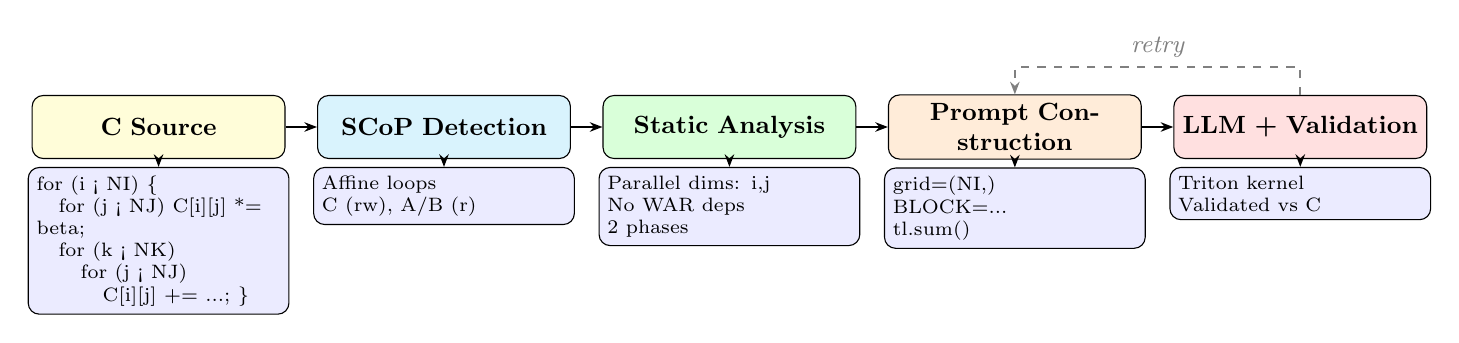
\begin{tikzpicture}[
  node distance=0.3cm and 0.35cm,
  box/.style={
    draw, rounded corners, text width=3.0cm, align=center,
    font=\small, minimum height=0.8cm, inner sep=3pt
  },
  io/.style={
    draw, rounded corners, fill=blue!8, text width=3.1cm,
    align=left, font=\scriptsize, inner sep=3pt
  },
  arr/.style={-{Stealth[length=1.6mm]}, thick}
]

% Stage 0
\node[box, fill=yellow!15] (source) {\textbf{C Source}};
\node[io, below=0.1cm of source] (srccode) {%
for (i < NI) \{\\
\quad for (j < NJ) C[i][j] *= beta;\\
\quad for (k < NK)\\
\quad\quad for (j < NJ)\\
\quad\quad\quad C[i][j] += ...; \}};

% Stage 1
\node[box, fill=cyan!15, right=0.4cm of source] (extract) {\textbf{SCoP Detection}};
\node[io, below=0.1cm of extract] (extout) {%
Affine loops\\
C (rw), A/B (r)};

% Stage 2
\node[box, fill=green!15, right=0.4cm of extract] (analysis) {\textbf{Static Analysis}};
\node[io, below=0.1cm of analysis] (anaout) {%
Parallel dims: i,j\\
No WAR deps\\
2 phases};

% Stage 3
\node[box, fill=orange!15, right=0.4cm of analysis] (prompt) {\textbf{Prompt Construction}};
\node[io, below=0.1cm of prompt] (promptout) {%
grid=(NI,)\\
BLOCK=...\\
tl.sum()};

% Stage 4
\node[box, fill=red!12, right=0.4cm of prompt] (llm) {\textbf{LLM + Validation}};
\node[io, below=0.1cm of llm] (llmout) {%
Triton kernel\\
Validated vs C};

% Horizontal arrows
\draw[arr] (source.east) -- (extract.west);
\draw[arr] (extract.east) -- (analysis.west);
\draw[arr] (analysis.east) -- (prompt.west);
\draw[arr] (prompt.east) -- (llm.west);

% Vertical arrows
\draw[arr] (source) -- (srccode);
\draw[arr] (extract) -- (extout);
\draw[arr] (analysis) -- (anaout);
\draw[arr] (prompt) -- (promptout);
\draw[arr] (llm) -- (llmout);

% Compact retry loop
\draw[arr, dashed, gray]
  (llm.north) -- ++(0,0.35)
  -| node[pos=0.25, above, font=\small\itshape] {retry}
  (prompt.north);

\end{tikzpicture}
\caption{The \sysname workflow.}
\label{fig:pipeline}
\end{figure*}

\sysname is implemented in approximately 14K lines of Python, using \pet/isl for polyhedral analysis and LLVM~17 for fallback dependence analysis.
Figure~\ref{fig:pipeline} depicts the workflow of \sysname using \texttt{gemm} as a running example. Given the source program (i.e., a C source file in this work), \sysname automatically identifies optimisation candidates and translates them into the target language (i.e., Triton kernels in this work). The \sysname pipeline consists of five stages: loop nest extraction, static analysis, prompt construction, LLM-based generation, and iterative refinement, described as follows. 
\subsection{Loop Nest Extraction}
The current implementation of \sysname targets loop-level code translation. It leverages \pet's Static Control Part (SCoP) detection~\cite{verdoolaege2012polyhedral} to identify affine loop nests suitable for transformation. It scans each function and selects regions where loop bounds and memory accesses are affine in loop iterators and parameters, requiring no manual annotations.
For example, for \texttt{gemm} in Figure~\ref{fig:pipeline} , \pet extracts a SCoP covering the full loop nest and produces a polyhedral representation including iteration domains, access relations, and loop schedules. This representation provides a precise and structured basis for subsequent dependence analysis.

\subsection{Static Analysis}
\sysname performs dependence-driven analysis to derive constraints that govern correct parallelization and code generation. It first identifies parallelizable loop dimensions with explicit validity conditions. In \texttt{gemm}, both \texttt{i} and \texttt{j} are parallelizable since updates to \texttt{C[i][j]} do not introduce cross-iteration conflicts. It then computes write-after-read (WAR) dependences using exact polyhedral analysis to determine whether in-place updates are safe. For \texttt{gemm}, no WAR dependences are present. Finally, it detects multi-phase computation patterns. In this case, beta scaling and matrix multiplication form two phases that share the array \texttt{C}, which affects kernel structuring.
When polyhedral analysis is not applicable (e.g., due to non-affine accesses), \sysname falls back to LLVM's \texttt{DependenceAnalysis} to conservatively infer dependence-carrying loops.

\subsection{Prompt Construction}
\sysname translates analysis results into structured guidance that constrains LLM generation. This step bridges compiler analysis and neural code synthesis. The guidance encodes: (i) valid and invalid parallelization choices with explicit mapping to execution grids, (ii) dependence-aware update strategies (in-place, clone, or sequential), (iii) phase decomposition for correctness, (iv) reduction patterns mapped to Triton primitives (e.g., \texttt{tl.sum()}, \texttt{tl.dot()}), and (v) required synchronization for cross-iteration or cross-phase dependences. This structured representation reduces ambiguity in the prompt and steers the LLM toward semantically correct and performant implementations.

\subsection{Generation and Iterative Refinement}

Given the constructed prompt, \sysname invokes the LLM (Claude Sonnet~4~\cite{anthropic2025claude} in this work) to generate the target code. The generated kernel is validated against the source program (compiled by LLVM in our case) using identical test inputs and FP32 tolerance checks. On validation failure, \sysname classifies the error and issues a targeted retry prompt. This process repeats for up to a fixed number of attempts (10 in this work), with a context reset after the sixth attempt to mitigate error accumulation.





% \paragraph{Static Analysis.}
% \pet{} extracts a polyhedral representation from which we compute:
% (a)~\emph{parallelizable dimensions} with validity constraints---for
% \texttt{gemm}, both \texttt{i} and \texttt{j} are valid since
% \texttt{C[i][j]} is a same-location read/write;
% (b)~\emph{WAR dependences} via exact polyhedral dependence
% analysis---\texttt{gemm} has none, so in-place update is safe;
% (c)~\emph{multi-phase decomposition}---the beta-scaling and
% matrix-multiply are two phases sharing array~\texttt{C}.
% When \pet{} cannot handle a construct (e.g., non-affine subscripts),
% we fall back to LLVM's \texttt{DependenceAnalysis} pass, parsing
% direction vectors to determine which loop levels carry dependences.

% \paragraph{Prompt Construction.}
% Analysis results are translated into five categories of structured
% natural-language guidance appended to the LLM prompt:

% \emph{Parallelization}: Each dimension is classified as valid,
% invalid (with reason), or reduction-safe.  For \texttt{gemm}:
% ``\emph{Parallelize \texttt{j}: \texttt{grid=(NI,)},
% vectorize with \texttt{BLOCK=min(next\_pow2(NJ),\allowbreak128)}.}''

% \emph{WAR dependences}: No WAR (in-place), WAR with clone
% (\texttt{A.clone()}), or sequential (\texttt{grid=(1,)}).

% \emph{Multi-phase split}: Cross-phase write conflicts trigger
% splitting into separate kernel launches.

% \emph{Reductions}: Mapped to \texttt{tl.sum()}/\texttt{tl.dot()}.

% \emph{Stencil barriers}: Cross-phase data dependences within
% a CTA trigger \texttt{tl.debug\_barrier()} insertion.

% \paragraph{Generation and Refinement.}
% The prompt is sent to Claude Sonnet~4~\cite{anthropic2025claude}.
% Generated code is tested against a C reference (\texttt{-O0})
% on identical random inputs, compared element-wise with FP32
% tolerances.  On failure, the system classifies the error and
% constructs a targeted retry prompt (up to 10~attempts, with a
% context reset at attempt~6).

% \sysname is implemented in $\sim$14,000 lines of Python.
% The analysis frontend uses \pet{}/isl~\cite{verdoolaege2010isl}
% and LLVM~17 for fallback dependence analysis.

\section{Evaluation Setup}

\cparagraph{Platforms.}
All experiments are conducted on a GPU workstation equipped with an NVIDIA RTX~3090 GPU (24\,GB memory, 936\,GB/s memory bandwidth) and a dual-socket Intel Xeon Gold 5218R CPU (80 logical cores, $\sim$140\,GB/s memory bandwidth).
We use PyTorch~2.5.1, Triton~3.1.0, CUDA~12.4, and GCC~11.4.0. We use Claude Sonnet~4~\cite{anthropic2025claude} as the underlying LLM for code translation.

\cparagraph{Benchmarks.}
We evaluate on three benchmark suites:
(1)~\emph{PolyBench/C}~\cite{polybench}: 30 numerical kernels (stencils, linear algebra, data mining) at default sizes ($N$=60--120) and 8$\times$ scale ($N$=480--960);
(2)~\emph{TSVC}~\cite{callahan1988tsvc}: 151 loop kernels covering linear traversals, reductions, indirect addressing, and loop-carried dependences, benchmarked at 32\,MB and 3200\,MB per array ($N$=8M and 800M);
(3)~\emph{Application kernels}: 8 kernels from Rodinia (SRAD, lud, gaussian, lavaMD, hotspot, pathfinder) and ECP proxy applications (miniMD LJ~force, miniFE SpMV).

\cparagraph{Baselines.}
The primary comparison is against \emph{OMP~GPU}---OpenMP GPU offloading compiled by NVIDIA \texttt{nvc} with managed memory, running on the \emph{same} GPU as Triton.
This is the strongest baseline: it isolates the quality of LLM-generated Triton code from hardware differences, directly comparing two GPU programming models on identical hardware.
We additionally report results against \emph{OMP~CPU} (80-thread OpenMP on CPU) to quantify the GPU's architectural advantage, and \emph{ST} (single-threaded GCC \texttt{-O3}) as a conventional reference point.

\cparagraph{Evaluation methodology.}
All speedups measure kernel-only execution time with data pre-staged on the GPU, averaged over 10--50 iterations after warmup.
For the correctness ablation, we compare two LLM configurations: \emph{with analysis} (WA), where the prompt includes compiler-derived guidance, and \emph{no analysis} (NA), where the LLM receives only the C source code. This isolates the contribution of static analysis to generation quality.
%% ===================================================================
\section{Experimental Results}
\label{sec:eval}


\subsection{Polybench/C (30 Kernels)}

\begin{table}[t]
  \caption{Polybench/C results.  WA = with analysis, NA = no analysis.}
  \label{tab:results_1x}
  \centering\small
  \begin{tabular}{lcc}
    \toprule
    \textbf{Metric} & \textbf{WA} & \textbf{NA} \\
    \midrule
    Pass rate              & 30/30 (100\%) & 28/30 (93\%) \\
    Median speedup         & 2.15$\times$  & 1.06$\times$ \\
    Mean speedup           & 3.44$\times$  & 1.52$\times$ \\
    Kernels $>1\times$     & 20/30         & 14/28         \\
    \midrule
    \multicolumn{3}{l}{\emph{Head-to-head (28 common):}} \\
    WA wins ($>$10\% faster) & \multicolumn{2}{c}{12} \\
    NA wins ($>$10\% faster) & \multicolumn{2}{c}{6 (3 race conditions)}  \\
    Ties (within 10\%)       & \multicolumn{2}{c}{10}  \\
    \bottomrule
  \end{tabular}
\end{table}

Table~\ref{tab:results_1x} summarizes results at standard
(1$\times$) problem sizes.  All 30 kernels pass with analysis
guidance; without it, two stencil kernels fail due to
parallelizing dimensions with carried dependences.
The 2.15$\times$ median speedup is limited by Polybench's
small defaults ($N$\,=\,60--120), where GPU launch overhead
dominates.  Compute-bound kernels show strong speedups
(\texttt{heat\_3d}: 12.36$\times$, \texttt{deriche}:
7.44$\times$, \texttt{covariance}: 7.40$\times$).

Of 6 apparent NA wins, 3 (\texttt{lu}, \texttt{ludcmp}, \texttt{bicg})
contain confirmed race conditions---the NA code uses
\texttt{grid=(N,)} for LU decomposition where row~$i$ reads from
row~$k$ ($k<i$) that may not yet be computed by its CTA, producing up
to $10^{33}$ variation across runs.  The remaining 3 NA wins reflect
nondeterministic LLM code quality, not structural differences.

\paragraph{Scaling.}

\begin{table}[t]
  \caption{Polybench scaling: 1$\times$ to 8$\times$ problem sizes
    ($N$: 60$\to$480, matrices: 120$\to$960).
    ``ST'' = single-threaded C; ``OMP'' = 80-thread OpenMP.}
  \label{tab:results_8x}
  \centering\small
  \begin{tabular}{lccc}
    \toprule
    \textbf{Metric} & \textbf{1$\times$} & \textbf{8$\times$ (ST)} & \textbf{8$\times$ (OMP)} \\
    \midrule
    Pass rate          & 30/30        & 30/30         & 30/30        \\
    Benchmarked        & 30           & 25$^*$        & 25$^*$       \\
    Median speedup     & 2.15$\times$ & 30.73$\times$ & 8.57$\times$ \\
    Kernels $>1\times$ & 20/30        & 21/25         & 20/25        \\
    \bottomrule
    \multicolumn{4}{l}{\scriptsize $^*$5 sequential kernels timeout during benchmark.}
  \end{tabular}
\end{table}

At 8$\times$ sizes (Table~\ref{tab:results_8x}), median speedup
rises to 30.73$\times$ over single-threaded C.  Against 80-thread
OpenMP, the GPU still achieves 8.57$\times$ median, confirming
genuine advantage beyond CPU parallelism.  Five sequential kernels
time out during benchmark (\texttt{grid=(1,)}).

\paragraph{Guidance Impact.}

\begin{table}[t]
  \caption{Impact of analysis-triggered guidance categories.
    ``Before'' and ``After'' are speedups at 1$\times$ sizes
    except where noted.}
  \label{tab:guidance_fixes}
  \centering\small
  \begin{tabular}{llcc}
    \toprule
    \textbf{Guidance} & \textbf{Kernel} & \textbf{Before} & \textbf{After} \\
    \midrule
    Multi-phase split      & correlation & 0.19$\times$ & 2.50$\times$ \\
    WAR sequential         & nussinov    & FAIL          & PASS         \\
    Triangular grid        & lud$^\dagger$ & 0.14$\times$ & 13.18$\times$ \\
    Fused reductions       & bicg        & 1.04$\times$ & 3.51$\times$ \\
    Stencil barriers       & jacobi\_1d  & 0.13$\times$ & 1.78$\times$ \\
    IIR phase fusion       & deriche     & 0.28$\times$ & 7.19$\times$ \\
    Tridiag.\ sweep        & adi         & 0.24$\times$ & 2.27$\times$ \\
    \bottomrule
    \multicolumn{4}{l}{\scriptsize $^\dagger$Rodinia benchmark.}
  \end{tabular}
\end{table}

Table~\ref{tab:guidance_fixes} shows the impact of individual
guidance categories, each triggered by analysis properties
(e.g., cross-phase dependences, triangular patterns).
The largest gains come from multi-phase decomposition
(correlation: 13$\times$) and triangular grid
(lud: 94$\times$).

\paragraph{Limitations.}
Ten kernels achieve $<$1$\times$ at standard sizes: five are
inherently sequential (loop-carried dependences limit parallelism),
and two (\texttt{jacobi\_2d}, \texttt{fdtd\_2d}) suffer from
kernel launch overhead at small $N$---at 8$\times$ sizes they reach
36.82$\times$ and 15.43$\times$.


\subsection{TSVC (151 Kernels)}
\label{sec:tsvc}

We apply \sysname to 151 TSVC~\cite{callahan1988tsvc} kernels
covering linear traversals, reductions, indirect addressing,
and loop-carried dependences.

\begin{table}[t]
  \caption{TSVC results at three data sizes.  ``ST'' = single-threaded
    C (\texttt{-O2}), ``OMP'' = OpenMP C (\texttt{-O2 -fopenmp},
    80~threads). Pass rate: 150/151 (99.3\%).}
  \label{tab:tsvc}
  \centering\small
  \begin{tabular}{lcc}
    \toprule
    & \textbf{32\,MB} & \textbf{3200\,MB} \\
    \midrule
    Per-array size     & 32\,MB & 3.2\,GB \\
    Parallelizable$^*$ & 27/150 & 15/150  \\
    \midrule
    Tri/ST median      & 67.1$\times$ & 73.2$\times$ \\
    Tri/OMP CPU median & 10.7$\times$ & 14.2$\times$ \\
    Tri/OMP GPU median & 1.02$\times$ & ---           \\
    \bottomrule
    \multicolumn{3}{l}{\scriptsize $^*$Serial/2D kernels excluded at large sizes.}
  \end{tabular}
\end{table}

Table~\ref{tab:tsvc} shows results at realistic data sizes.
\sysname passes 150/151 (99.3\%), 120 on first attempt.
At 32\,MB, LLM-generated Triton achieves 67$\times$ (ST)
and 10.7$\times$ (80-thread OMP CPU).  Crucially, Triton
achieves \textbf{1.02$\times$ vs.\ OpenMP GPU offloading}
(\texttt{nvc~-mp=gpu}) on the \emph{same} GPU, showing the
LLM produces code matching a production compiler.


\subsection{Application Kernels}
\label{sec:realworld}

\begin{table}[t]
  \caption{Application kernel results.  ``---'' = NA failed all attempts.}
  \label{tab:realworld}
  \centering\small
  \begin{tabular}{llcc}
    \toprule
    \textbf{Source} & \textbf{Kernel} & \textbf{WA} & \textbf{NA} \\
    \midrule
    Rodinia & SRAD       & 24.86$\times$ & 3.50$\times$ \\
    Rodinia & lud        & 13.18$\times$ & 15.52$\times$ \\
    Rodinia & gaussian   & 3.35$\times$  & 3.61$\times$ \\
    Rodinia & lavaMD     & 1.47$\times$  & 0.56$\times$ \\
    Rodinia & hotspot    & 1.05$\times$  & 1.22$\times$ \\
    Rodinia & pathfinder & 0.11$\times$  & --- \\
    \midrule
    miniMD  & LJ force   & 25.82$\times$ & 23.00$\times$ \\
    miniFE  & SpMV       & 8.95$\times$  & 7.27$\times$ \\
    \bottomrule
  \end{tabular}
\end{table}

To evaluate generalization beyond synthetic benchmarks, we apply
\sysname to 6 Rodinia kernels~\cite{che2009rodinia} and 2 ECP proxy
application kernels~\cite{heroux2009mantevo}---CSR sparse matrix-vector
multiply (SpMV) from miniFE and Lennard-Jones force computation from
miniMD (Table~\ref{tab:realworld}).  All 8 pass correctness with
analysis guidance (6 on the first attempt).

SRAD (24.9$\times$) has three computational phases per iteration;
the analysis detects cross-phase dependences and recommends splitting
into separate kernels with parallel grids, yielding 7.1$\times$
improvement over the NA baseline (3.5$\times$).
The LJ force kernel from miniMD computes pairwise forces using a full
neighbor list; the outer loop over atoms is embarrassingly parallel.
With analysis guidance the LLM iterates only actual neighbors
(25.8$\times$), while the NA version wastes cycles on padded entries
(23.0$\times$).
lavaMD improves from 0.56$\times$ (NA) to 1.47$\times$ (WA) as
analysis identifies the parallelizable particle dimension, while the
NA baseline fails with type-mismatch errors on 4 of 5 attempts.
SpMV achieves 8.95$\times$ with analysis vs.\ 7.27$\times$ without,
as guidance helps select better block sizes for the row-parallel pattern.
For lud and hotspot, both versions produce near-identical Triton
times; the speedup differences reflect C reference timing variance.



%% ===================================================================
\section{Related Work}
\label{sec:related}

\paragraph{LLM Code Generation for GPUs.}
Chen et al.~\cite{chen2024chatgpt} evaluate ChatGPT on CUDA kernel
generation, finding frequent correctness issues including data races and
incorrect memory management.
KernelBench~\cite{ouyang2024kernelbench} benchmarks LLM-generated
Triton/CUDA on 250 tasks, reporting 20--40\% functional correctness
without guidance.  Our work differs fundamentally: rather than relying
on the LLM's implicit knowledge of parallelism, we provide explicit
compiler-derived constraints, achieving 100\% correctness on
Polybench/C and 99\% on TSVC.

\paragraph{Polyhedral Compilation and Auto-Scheduling.}
Polyhedral frameworks such as Pluto~\cite{bondhugula2008pluto} and
PPCG~\cite{verdoolaege2013ppcg} automatically generate parallel code
from affine loop nests.  PPCG targets CUDA directly but is limited to
affine programs and produces low-level code that lacks Triton's
block-level optimizations (automatic memory coalescing, shared memory
tiling).  TVM~\cite{chen2018tvm} and Halide~\cite{ragan2013halide}
use auto-scheduling with learned cost models for tensor operations.
\sysname is complementary: rather than replacing the compiler,
it uses polyhedral analysis to extract \emph{what} parallelism is
safe, then delegates the \emph{how} to the LLM, which can handle
non-affine constructs, irregular access patterns, and high-level
Triton abstractions that polyhedral compilers cannot target directly.


%% ===================================================================
\section{Conclusion}
\label{sec:conclusion}
We have presented \sysname, a system that combines compiler-based analysis with LLM-based kernel generation for accelerators. By translating parallelization constraints, dependence information, and memory access patterns into structured prompts, \sysname enables LLMs to generate correct and efficient Triton kernels from C programs.

\sysname achieves near-perfect correctness (30/30 PolyBench/C, 150/151 TSVC) and generates Triton code that matches production compiler quality: on TSVC at 32\,MB, LLM-generated Triton achieves 1.02$\times$ median vs.\ OpenMP GPU offloading (\texttt{nvc}) on the same GPU. It generalizes to 8 application kernels from Rodinia and ECP proxy apps.
Ablation results show that analysis-guided prompting is essential for correctness, preventing failures and exposing latent race conditions in unguided generation. Future work includes extending to non-affine programs and integrating autotuning for parameter selection.

%% ===================================================================
%% References
\bibliographystyle{ACM-Reference-Format}
\begin{thebibliography}{99}

\bibitem{tillet2019triton}
P.~Tillet, H.~T. Kung, and D.~Cox.
\newblock Triton: An intermediate language and compiler for tiled neural
  network computations.
\newblock In \emph{Proc. MAPL}, 2019.

\bibitem{chen2024chatgpt}
Y.~Chen, S.~Huang, D.~Zheng, et~al.
\newblock {ChatGPT} for {CUDA} programming: Evaluating {LLM}-generated {GPU}
  code.
\newblock \emph{arXiv preprint arXiv:2404.12000}, 2024.

\bibitem{ouyang2024kernelbench}
A.~Ouyang, S.~Zheng, et~al.
\newblock {KernelBench}: Can {LLMs} write efficient {GPU} kernels?
\newblock \emph{arXiv preprint arXiv:2404.12489}, 2024.

\bibitem{verdoolaege2012polyhedral}
S.~Verdoolaege and T.~Grosser.
\newblock Polyhedral extraction tool.
\newblock In \emph{Proc. IMPACT}, 2012.

\bibitem{llvm}
C.~Lattner and V.~Adve.
\newblock {LLVM}: A compilation framework for lifelong program analysis \&
  transformation.
\newblock In \emph{Proc. CGO}, 2004.

\bibitem{polybench}
L.-N. Pouchet.
\newblock Polybench/C: The polyhedral benchmark suite, version 4.2.1.
\newblock \url{https://web.cs.ucla.edu/~pouchet/software/polybench/}, 2016.

\bibitem{anthropic2025claude}
Anthropic.
\newblock Claude {Sonnet} 4 model card.
\newblock \url{https://www.anthropic.com/claude}, 2025.

\bibitem{verdoolaege2010isl}
S.~Verdoolaege.
\newblock isl: An integer set library for the polyhedral model.
\newblock In \emph{Proc. ICMS}, 2010.

\bibitem{chen2018tvm}
T.~Chen, T.~Moreau, Z.~Jiang, et~al.
\newblock {TVM}: An automated end-to-end optimizing compiler for deep
  learning.
\newblock In \emph{Proc. OSDI}, 2018.

\bibitem{ragan2013halide}
J.~Ragan-Kelley, C.~Barnes, A.~Adams, et~al.
\newblock Halide: A language and compiler for optimizing parallelism,
  locality, and recomputation in image processing pipelines.
\newblock In \emph{Proc. PLDI}, 2013.

\bibitem{bondhugula2008pluto}
U.~Bondhugula, A.~Hartono, J.~Ramanujam, and P.~Sadayappan.
\newblock A practical automatic polyhedral parallelizer and locality
  optimizer.
\newblock In \emph{Proc. PLDI}, 2008.

\bibitem{verdoolaege2013ppcg}
S.~Verdoolaege, J.~Carlos~Juega, A.~Cohen, et~al.
\newblock Polyhedral parallel code generation for {CUDA}.
\newblock \emph{ACM TACO}, 9(4), 2013.

\bibitem{che2009rodinia}
S.~Che, M.~Boyer, J.~Meng, et~al.
\newblock Rodinia: A benchmark suite for heterogeneous computing.
\newblock In \emph{Proc. IISWC}, 2009.

\bibitem{heroux2009mantevo}
M.~A.~Heroux, D.~W.~Doerfler, P.~S.~Crozier, et~al.
\newblock Improving performance via mini-applications.
\newblock Sandia National Laboratories Technical Report SAND2009-5574, 2009.

\bibitem{callahan1988tsvc}
D.~Callahan, J.~Dongarra, and D.~Levine.
\newblock Vectorizing compilers: A test suite and results.
\newblock In \emph{Proc. Supercomputing}, 1988.

\end{thebibliography}

\end{document}
